\documentclass[UKenglish]{article}  %% ... or USenglish or norsk or nynorsk
\usepackage[utf8]{inputenc}           %% ... or latin1 or applemac
\usepackage[T1]{fontenc,url}
\urlstyle{sf}
\usepackage{tikz,babel,textcomp,csquotes,pgf-umlsd,varioref,graphicx}
\usetikzlibrary{arrows, shadows}
\title{Project 1}        %% ... or whatever
         %% ... if any
\author{Aulon Mujaj, Henning Lund-Hanssen, Espen Jones}                      %% ... or whoever 

\begin{document}
\maketitle{}

\section{Requirement 1 - Brief analysis}

\subsection{Brief description}

\subsection{Analysis}

\subsection{Non-functional tests}

\subsection{Test cases}

\section{Requirement 2 - In-depth metrics}

\subsection{Metrics at project level}
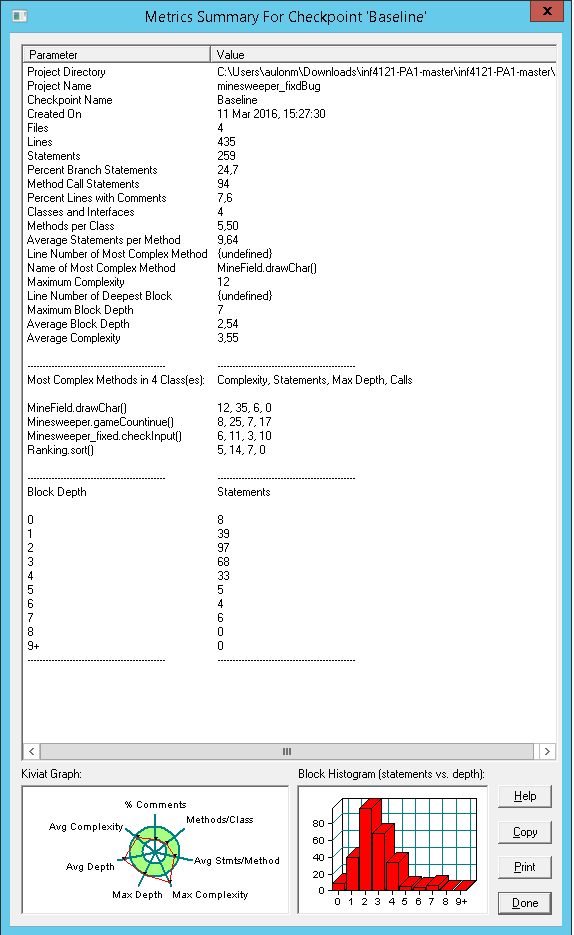
\includegraphics[height=8cm]{metric_summary}
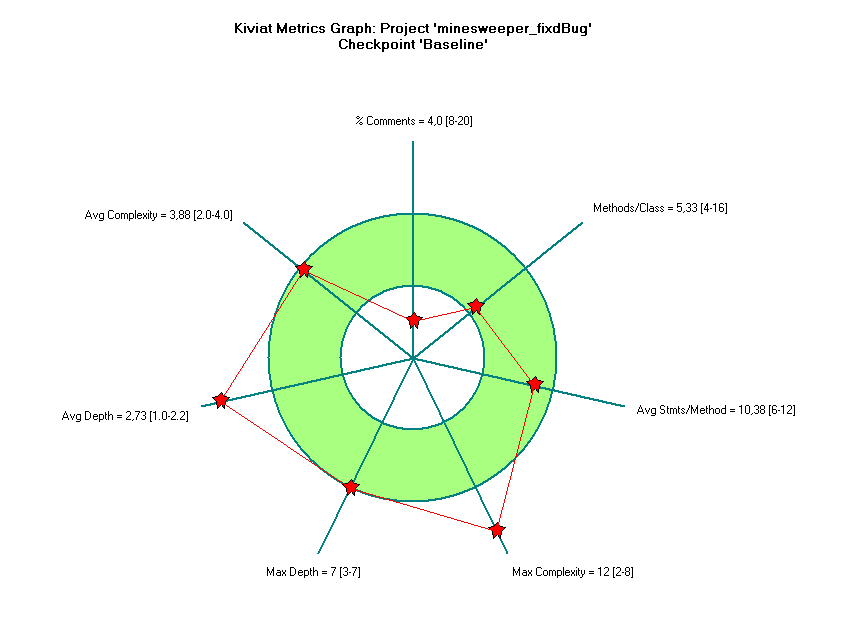
\includegraphics[height=8cm]{kiviat_diagram_baseline}
\begin{itemize}
\item What metrics do you spot for the whole project in the window Metrics Summary for Checkpoint? Write a brief description of the metrics. Try to explain their values (below what is expected, as expected or above the expected level). What metrics do you think need to change?\\
\item Which is the biggest file you have in your project by the number of lines of code? \\
MineField.java
\item Which is the file with most branches in your project?\\
\item Which is the file with most complex code? What metric did you choose to answer to this question?\\
Minesweeper.java
\end{itemize}

Write a little about each metric, maybe we'll only write about the 6 different metrics from the kiviat diagram, instead of each metric from the metric summary image?

If we choose to go only for the metrics from the kiviat diagram, then we'll only need to write about:\\
Avg complexity, avg depth, max depth, \% comments, methods/class, avg stats/method, max complexity\\

Statements:
Branch statements:
Method call statements:
Percent lines with comments:
Classes and Interfaces
Methods per class:
Average Statements per Method:
Name of Most complex methods
Maximum Complexity
Maximum Block Depth
Average Block Depth
Average Complexity
Most complext methods (complexity, statements, max depth, calls)
How many statements on each block depth



\subsection{Metrics at file level}
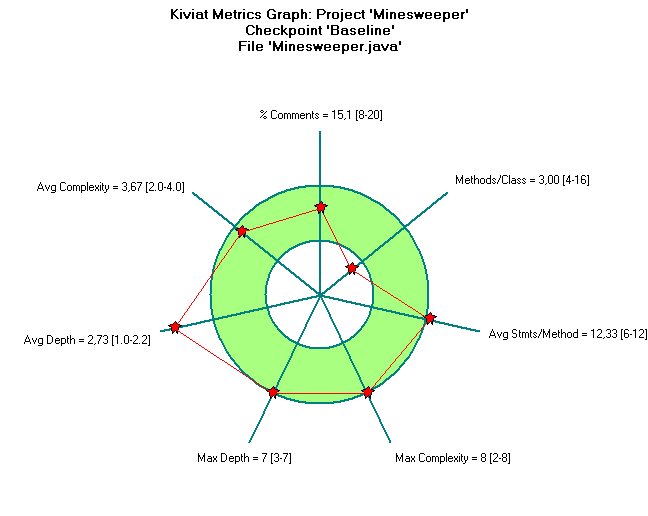
\includegraphics[height=8cm]{kiviat_diagram_minesweeper}
\begin{itemize}
\item How do you interpret the metrics applied on your file? How are they different the metrics you optained on the whole project, compared with the metrics ont his file?\\
\item Would you refactor (re-write) any of the methods you have in this file?
\end{itemize}
\section{Requirement 3 - Code improvement}

\subsection{Identification of metrics}

\subsection{Results from changes}

\subsection{Final remarks}

\end{document}
